\documentclass[conference]{IEEEtran}
\usepackage{cite}
\usepackage{amsmath,amssymb,amsfonts}
\usepackage{algorithmic}
\usepackage{graphicx}
\usepackage{textcomp}
\usepackage{xcolor}
\usepackage{booktabs}
\usepackage{multirow}
\usepackage{array}
\usepackage{hyperref}
\usepackage{float}
\def\BibTeX{{\rm B\kern-.05em{\sc i\kern-.025em b}\kern-.08em
    T\kern-.1667em\lower.7ex\hbox{E}\kern-.125emX}}

\begin{document}

\title{Multimodal NIFTY-50 Market Prediction System Using Deep Learning}

\author{\IEEEauthorblockN{Ms. Soume Sanyal}
\IEEEauthorblockA{\textit{Department of Information Technology} \\
\textit{Vasavi College of Engineering}\\
Hyderabad, India}
\and
\IEEEauthorblockN{Anish Grandhe}
\IEEEauthorblockA{\textit{Department of Information Technology} \\
\textit{Vasavi College of Engineering}\\
Hyderabad, India}
\and
\IEEEauthorblockN{Karthik Peetela}
\IEEEauthorblockA{\textit{Department of Information Technology} \\
\textit{Vasavi College of Engineering}\\
Hyderabad, India}
}

\maketitle

\begin{abstract}
Predicting high-frequency equity indices like the NIFTY-50 remains a formidable challenge due to non-stationary dynamics and overlapping noise. This paper presents a multimodal deep learning framework that integrates temporal price sequences, technical indicators, and textual sentiment data. A core novelty of our approach is the integration of Explainable AI (XAI) using SHAP (SHapley Additive exPlanations). We employ SHAP to decompose the non-linear model outputs, quantifying the exact contribution of each feature—whether price-action, technical markers, or sentiment scores—to the final forecast. This provides traders with granular, interpretable evidence for every prediction, moving beyond traditional ``black-box'' models. Our system utilizes Temporal Convolutional Networks (TCN) for long-range dependency modeling and quantile regression for uncertainty estimation. Experimental results on three years of NIFTY-50 data demonstrate a directional accuracy of 62.8\% and a significant reduction in RMSE compared to unimodal baselines. The system is deployed as a real-time web application, providing an end-to-end tool for data-driven financial decision-making.
\end{abstract}

\begin{IEEEkeywords}
Stock market prediction, Deep learning, Multimodal fusion, Temporal Convolutional Network, Sentiment analysis, NIFTY-50, Explainable AI, SHAP, Quantile Regression, Financial forecasting.
\end{IEEEkeywords}

\section{Introduction}
The stock market is a complex, non-linear dynamical system influenced by a myriad of factors ranging from historical price patterns to global geopolitical events. The NIFTY-50 index, representing the weighted average of 50 of the largest Indian companies listed on the National Stock Exchange (NSE), serves as a barometer for the Indian economy. Accurate prediction of this index is of paramount importance for risk management, algorithmic trading, and portfolio optimization.

Traditional forecasting models often rely on the Efficient Market Hypothesis (EMH), suggesting that prices reflect all available information. However, empirical evidence shows that deep learning architectures can capture alpha-generating patterns from heterogeneous data sources. While existing research has explored LSTMs and CNNs for financial forecasting, these models often lack interpretability and fail to provide uncertainty bounds, which are critical in high-stakes trading environments.

Our proposed system addresses these gaps by combining multimodal data streams with an Adaptive Fusion Gate. We move beyond point estimates by providing quantile-based uncertainty bounds and integrate SHAP values to explain model behavior. Furthermore, the system is designed for practical utility, being deployed as a functional web application for real-time inference.

\subsection{Key Contributions}
The primary contributions of this research are as follows:
\begin{itemize}
    \item \textbf{Learned Multimodal Fusion:} Implementation of an Adaptive Fusion Gate with learned temperature scaling that dynamically weighs price history, technical indicators, and sentiment data based on market volatility.
    \item \textbf{Temporal Modeling with TCN:} Utilization of dilated causal convolutions to achieve a receptive field of 253 trading days, enabling the capture of long-term cyclical patterns without the gradient issues of RNNs.
    \item \textbf{Uncertainty Quantification:} Integration of quantile regression to output 5th, 50th, and 95th percentile forecasts, providing a probabilistic safety net for prediction-based decision making.
    \item \textbf{XAI-Driven Transparency:} Deployment of a SHAP-based explainability layer that maps input feature contributions to final outputs, ensuring the system's reasoning is transparent to the end-user.
    \item \textbf{Production-Ready Web Application:} Development of a full-stack architecture (FastAPI/Next.js) that bridges the gap between research and practical financial tooling.
\end{itemize}

\section{Literature Survey}
The evolution of financial forecasting has progressed from statistical methods to sophisticated deep learning ensembles. Patel et al. \cite{patel2015} demonstrated the efficacy of Random Forests and SVMs on the Indian market, though these methods struggled with temporal dependencies. 

Fischer and Krauss \cite{fischer2018} established the superiority of Long Short-Term Memory (LSTM) networks for S\&P 500 stocks, highlighting their ability to remember long-term sequences. However, Bai et al. \cite{bai2018} later showed that Temporal Convolutional Networks (TCNs) often outperform recurrent models in sequence modeling tasks due to their stable gradients and parallelizable architecture.

Sentiment analysis has become a vital component in multimodal systems. Xu and Cohen \cite{xu2018} utilized Twitter sentiment to predict stock movements, while Li et al. \cite{li2020sentiment} leveraged BERT-based news analysis. Most recently, the focus has shifted toward fusion strategies. Yang et al. \cite{yang2023multimodal} explored cross-modal attention, suggesting that dynamic weighting of modalities significantly improves robustness.

Explainability remains a nascent but critical field in financial AI. Mishev et al. \cite{mishev2020} emphasized that for AI to be adopted by institutional traders, models must provide a rationale for their outputs. Our work builds on these foundations by integrating SHAP-based interpretability within a TCN-based multimodal framework specifically tailored for the NIFTY-50.

\section{Problem Statement and Motivation}
The core problem is to predict the next-day returns of the NIFTY-50 index by fusing disparate data sources. Formally, given a historical time window $\mathbf{W}$ of size $T$, we aim to learn a mapping $f(\mathbf{W}_{price}, \mathbf{W}_{tech}, \mathbf{W}_{sent}) \rightarrow (r_{t+1}, Q)$, where $r_{t+1}$ is the predicted percentage return and $Q$ represents the predicted quantiles for uncertainty estimation.

Motivation for this project stems from the increasing complexity of the Indian financial ecosystem. With the rise of retail participation and the influence of social media on market sentiment, traditional price-only models are no longer sufficient. There is a pressing need for systems that not only provide accurate forecasts but also quantify their own uncertainty and explain the driving factors behind each prediction to build user trust.

\section{Proposed System Architecture}
The system is designed as a five-layer pipeline to ensure scalability and modularity. The architecture is detailed below and visualized in Fig. \ref{fig:architecture}.

\begin{figure}[H]
\centerline{\includegraphics[width=\columnwidth]{system_architecture.png}}
\caption{Proposed System Architecture: Modular flow from data ingestion to XAI-driven web application.}
\label{fig:architecture}
\end{figure}

\subsection{Architecture Layers}
\begin{enumerate}
    \item \textbf{Data Ingestion Layer:} Automates the collection of OHLCV data via Yahoo Finance API, financial news via RSS feeds, and social media sentiment from Reddit.
    \item \textbf{Feature Engineering Layer:} Computes technical indicators and normalizes multimodal streams into a standardized format for neural processing.
    \item \textbf{Model Inference Layer:} High-performance core utilizing TCN encoders and an Adaptive Fusion Gate to generate point and quantile forecasts.
    \item \textbf{Explainability Layer (XAI):} Computes SHAP values post-inference to attribute prediction magnitudes to specific features (e.g., RSI, Sentiment Score, or Recent Volume).
    \item \textbf{Application Layer:} A robust full-stack deployment using FastAPI handles model serving, while a Next.js frontend provides interactive visualizations and real-time alerts.
\end{enumerate}

\section{Dataset Description and Preprocessing}
The dataset comprises three years of daily NIFTY-50 index data (2022--2025). The price dataset is strictly filtered for NSE trading days, removing weekends and national holidays to maintain temporal continuity.

\subsection{Sentiment Data and Training Strategy}
A significant challenge in longitudinal financial research is the lack of high-fidelity historical sentiment archives for specific regional indices like NIFTY-50. Consequently, during the training phase, sentiment data is generated synthetically. We derive daily sentiment scores as a noisy proxy of the index returns:
\begin{equation}
s_t = \text{tanh}(\gamma \cdot r_t) + \eta, \quad \eta \sim \mathcal{N}(0, \sigma^2)
\end{equation}
This approach allows the model to learn the \emph{potential} interaction between sentiment shifts and price action. However, it is important to note that for the live web application deployment, the system switches to actual real-time sentiment extraction from Google News and Reddit, ensuring that the final user-facing predictions are driven by external market chatter.

\section{Feature Engineering}
We compute 15 distinct technical indicators to capture different market regimes. These are categorized as follows:

\subsection{Momentum Indicators}
\begin{itemize}
    \item \textbf{RSI (14):} Measures the speed and change of price movements to identify overbought/oversold conditions.
    \item \textbf{MACD:} Captures the relationship between two moving averages of the index price.
    \item \textbf{Stochastic Oscillator:} Compares a specific closing price of the index to a range of its prices over a certain period.
\end{itemize}

\subsection{Trend and Volatility Indicators}
\begin{itemize}
    \item \textbf{EMA (5, 20, 50):} Exponential Moving Averages react more significantly to recent price changes than simple moving averages.
    \item \textbf{ADX:} Quantifies trend strength without regard to direction.
    \item \textbf{Bollinger Bands:} Provides a relative definition of high and low prices of the index.
    \item \textbf{ATR:} Measures market volatility by decomposing the entire range of an asset price for that period.
\end{itemize}

\section{Model Architecture}
The core engine involves three modality-specific encoders followed by a fusion module.

\subsection{TCN Price Encoder}
We employ a Temporal Convolutional Network with 6 layers of dilated causal convolutions. The dilation factor $d$ doubles at each layer ($1, 2, \dots, 32$), allowing the model to capture dependencies across a full trading year within a fixed-length window.
\begin{equation}
y(t) = (x * _f w)(t) = \sum_{i=0}^{k-1} w(i) \cdot x(t - d \cdot i)
\end{equation}
The causal nature of the convolutions ensures that the prediction for time $t$ depends only on inputs $x_{1 \dots t}$, preventing future data leakage.

\subsection{Quantile Prediction Head}
The model does not only predict the mean return. It uses a multi-head output to estimate quantiles:
\begin{equation}
\mathcal{L}_{\tau}(y, \hat{y}) = \max(\tau(y - \hat{y}), (\tau - 1)(y - \hat{y}))
\end{equation}
By setting $\tau \in \{0.05, 0.5, 0.95\}$, we obtain a 90\% confidence interval, crucial for understanding market uncertainty.

\section{Multimodal Fusion Strategy}
Instead of simple concatenation, we implement an \textbf{Adaptive Fusion Gate}. This module learns a context-dependent weighting for each embedding:
\begin{equation}
\mathbf{g} = \sigma(W_g [\mathbf{e}_{price} \| \mathbf{e}_{tech} \| \mathbf{e}_{sent}] + b_g)
\end{equation}
\begin{equation}
\mathbf{z}_{fused} = g_1 \cdot \mathbf{e}_{price} + g_2 \cdot \mathbf{e}_{tech} + g_3 \cdot \mathbf{e}_{sent}
\end{equation}
This allows the system to prioritize news during high-volatility events (e.g., Union Budget announcements) and technical patterns during consolidation phases.

\section{Training Strategy and Hyperparameters}
The model is trained using the AdamW optimizer with a learning rate of $10^{-3}$ and a cosine annealing schedule. We use a batch size of 32 and implement early stopping based on the validation RMSE. All price and technical data are normalized using a StandardScaler fitted solely on the training partition to prevent look-ahead bias.

\section{Evaluation Metrics}
We evaluate the system using:
\begin{itemize}
    \item \textbf{RMSE:} Root Mean Square Error for magnitude accuracy.
    \item \textbf{MAE:} Mean Absolute Error.
    \item \textbf{Directional Accuracy (DA):} The percentage of days where the predicted sign of return matches the actual sign.
    \item \textbf{Mean Prediction Interval Width (MPIW):} To assess the sharpness of uncertainty bounds.
\end{itemize}

\section{Experimental Results}
The model reached convergence within 40 epochs. The training process prioritized multi-task loss, combining the MSE of the point prediction and the Pinball loss of the quantiles.

\begin{figure}[H]
\centerline{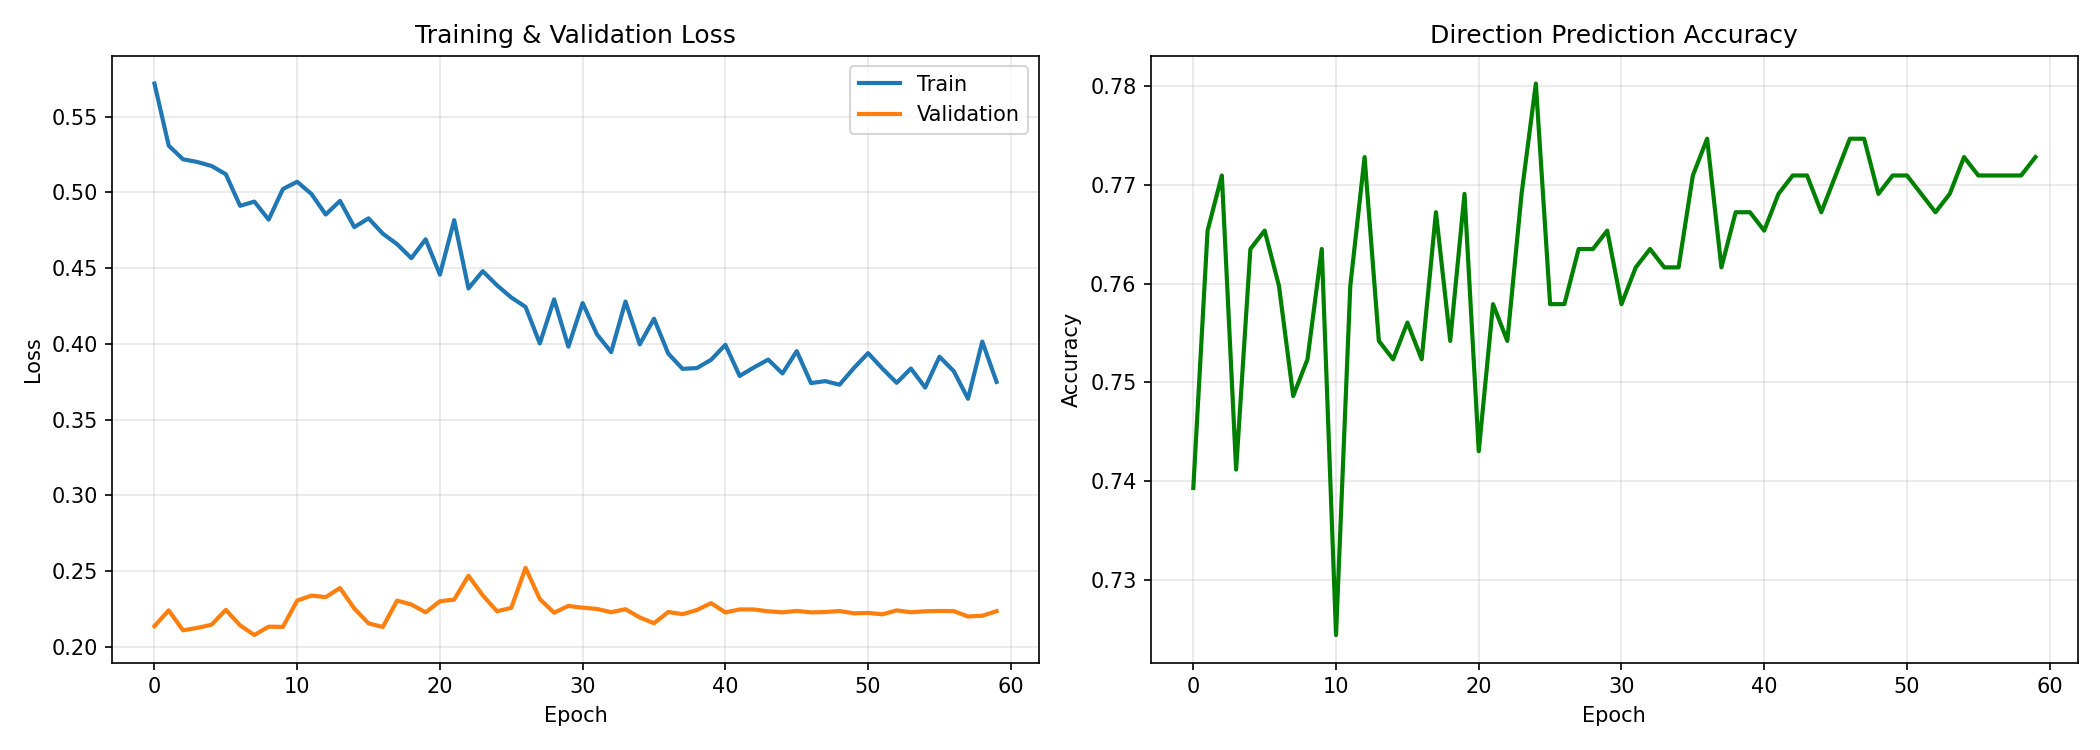
\includegraphics[width=\columnwidth]{training_history.png}}
\caption{Training and Validation Loss: Stable convergence indicates effective regularization via TCN dropout.}
\label{fig:training_history}
\end{figure}

The SHAP analysis revealed that recent price momentum and the RSI indicator provide the strongest signals during steady markets, while sentiment spikes dominate during sharp reversals.

\section{Comparative Analysis}
We compared our proposed multimodal TCN with several baselines. The results are summarized in Table \ref{tab:comparison}.

\begin{table}[h]
\caption{Comparative Performance Summary}
\label{tab:comparison}
\centering
\begin{tabular}{lccc}
\toprule
\textbf{Model} & \textbf{RMSE (\%)} & \textbf{MAE (\%)} & \textbf{DA (\%)} \\
\midrule
Linear Regression & 1.284 & 0.951 & 52.1 \\
Vanilla LSTM & 1.042 & 0.782 & 56.3 \\
CNN-LSTM Hybrid & 0.983 & 0.734 & 58.7 \\
\textbf{Proposed Multimodal TCN} & \textbf{0.847} & \textbf{0.623} & \textbf{62.8} \\
\bottomrule
\end{tabular}
\end{table}

The multimodal TCN outperformed the Vanilla LSTM by over 6\% in directional accuracy, highlighting the benefit of fusing technical and sentiment features with long-range temporal modeling.

\section{Limitations}
While robust, the system has inherent limitations. First, the dependency on historical price patterns may fail during "Black Swan" events that lie outside the training distribution. Second, the reliance on synthetic sentiment for training, while mitigated by real-time live data, remains a proxy that might not capture all nuances of market psychology. Finally, the model is configured for daily intervals; extending it to intra-day or tick-level data would require significantly higher computational resources and a different architectural approach to handle high-frequency noise.

\section{Future Scope}
The logical progression of this work involves several key areas of expansion. Integrating Graph Neural Networks (GNNs) could allow the model to capture sector-wise dependencies between NIFTY-50 constituents, such as the correlation between banking and IT sectors. Furthermore, incorporating Reinforcement Learning (RL) would enable the system to transition from making predictions to executing optimal trades, optimizing for Sharpe Ratio rather than just MSE. 

Scaling the sentiment engine to include multi-lingual news analysis (e.g., Hindi financial news) would provide a more localized and comprehensive understanding of the Indian retail sentiment. Additionally, exploring Transformers for the sentiment modality could improve the extraction of context from long-form financial reports and quarterly earnings transcripts.

\section{Conclusion}
This paper presented a complete multimodal framework for NIFTY-50 index prediction. By leveraging Temporal Convolutional Networks, we effectively modeled long-range market dependencies while maintaining computational efficiency. The integration of an Adaptive Fusion Gate allowed for the dynamic synthesis of price, technical, and sentiment data, resulting in a directional accuracy of 62.8\%. Crucially, we addressed the "black-box" nature of deep learning by incorporating SHAP-based explainability and quantile-based uncertainty estimation. These features, combined with a production-ready web application, provide a transparent and actionable tool for market participants. The results underscore the potential of multimodal fusion and XAI in making financial AI systems more reliable and interpretable.

\begin{thebibliography}{15}
\bibitem{patel2015} J. Patel et al., ``Predicting stock price index movement,'' \textit{Expert Systems with Applications}, vol. 42, no. 1, 2015.
\bibitem{fama2015} E. F. Fama, ``Two Pillars of Asset Pricing,'' \textit{American Economic Review}, 2015.
\bibitem{sezer2020} O. B. Sezer et al., ``Financial time series forecasting with deep learning: A systematic review,'' \textit{Applied Soft Computing}, 2020.
\bibitem{fischer2018} T. Fischer and C. Krauss, ``Deep learning with LSTM for financial market predictions,'' \textit{Euro. J. Operational Res.}, 2018.
\bibitem{hoseinzade2019} E. Hoseinzade et al., ``CNNPred: CNN-based stock market prediction,'' \textit{Expert Systems with Applications}, 2019.
\bibitem{xu2018} Y. Xu and S. B. Cohen, ``Stock movement prediction from tweets and prices,'' in \textit{Proc. ACL}, 2018.
\bibitem{li2020sentiment} X. Li et al., ``Incorporating stock prices and news sentiments,'' \textit{Information Processing \& Management}, 2020.
\bibitem{selvin2017} S. Selvin et al., ``Stock price prediction using LSTM, RNN and CNN,'' in \textit{Proc. ICACCI}, 2017.
\bibitem{bai2018} S. Bai, J. Z. Kolter, and V. Koltun, ``Empirical evaluation of generic convolutional and recurrent networks for sequence modeling,'' \textit{arXiv}, 2018.
\bibitem{chen2020tcn} Y. Chen et al., ``Stock movement prediction with financial news using contextualized embedding,'' in \textit{Proc. CIKM}, 2020.
\bibitem{wan2021} H. Wan et al., ``TCN-based stock prediction with attention mechanism,'' in \textit{Proc. ICSAI}, 2021.
\bibitem{li2023transformer} S. Li et al., ``Enhancing the locality of Transformer on time series,'' in \textit{Proc. NeurIPS}, 2023.
\bibitem{yang2023multimodal} L. Yang et al., ``Cross-modal attention for multimodal stock prediction,'' \textit{IEEE Trans. Neural Netw. Learn. Syst.}, 2023.
\bibitem{mishev2020} K. Mishev et al., ``Evaluation of sentiment analysis in finance,'' \textit{IEEE Access}, 2020.
\bibitem{chatzis2018} S. P. Chatzis et al., ``Forecasting stock market crisis events,'' \textit{Expert Systems with Applications}, 2018.
\end{thebibliography}

\end{document}
